\section{Evaluation}

\subsection{Data Collection Tools}
\subsubsection{Data Collection Software}
The software used to collect data for this experiment is the AppMon logging mobile application 
for the Android phone. 
The AppMon application logs data from various smartphone sensors, including the following:
\begin{enumerate}
\item Accelerometer
\item Number of unlocks
\item Number of screen touches
\item Number of times the screen turns on and off
\end{enumerate}

In our project, we will be using data from the sensors
to create features in order to classify and predict the location of the phone. 

The app collects accelerometer readings (X, Y, Z directions) in units of $m/s^2$ every 10ms.
It also registers the timestamp at which various trigger events occur (e.g. phone unlocks, screen on, etc.)

\subsubsection{Phones}
We used two phones for the purpose of diary studies and collecting data for creating the classifiers.
One phone was a Nexus 5 and the other was a Nexus 5x


\subsection {Diary Study}
To obtain data for training and validation, three `diary studies' were performed, all by the same participant.

In each study, the participant would carry the phone around with the aforementioned app running and undergo a daily routine.
Whenever a change of state occured, the participant would record the time (according to the phone) and the new state.

The first diary study was performed for a total of roughly 14.5 hours using the Nexus 5x which was also used as the source of training as well as validation data.
The second and third diary studies were performed using the Nexus 5.
This data was used to check for cross-phone validation.


The distribution of the states during the diary study are shown below:


\begin{table}[h]
\caption{Distribution of States for Diary Study 1 (Nexus 5x)}\label{tab:diary1} \centering
\begin{tabular}{ |c|c|c| } 
 \hline
 Table & 9.29 hours & 0.635\%  \\ 
 Pocket & 0.49 hours & 0.034\% \\ 
 Backpack &  4.26 hours  &  0.292\% \\ 
 Hand & 0.58 hours  & 0.039\% \\
 \hline
\end{tabular}
\end{table}

\begin{table}[h]
\caption{Distribution of States for Diary Study 2 (Nexus 5)}\label{tab:diary1} \centering
\begin{tabular}{ |c|c|c| } 
 \hline
 Table & 2.85 & 0.400\%  \\ 
 Pocket & 1.45 & 0.204\% \\ 
 Backpack &  0.15 hours  &  0.021\% \\ 
 Hand & 2.67 hours  & 0.375\% \\
 \hline
\end{tabular}
\end{table}

\begin{table}[h]
\caption{Distribution of States for Diary Study 3 (Nexus 5)}\label{tab:diary1} \centering
\begin{tabular}{ |c|c|c| } 
 \hline
 Table & 0.44 & 0.061\%  \\ 
 Pocket & 0.60 & 0.085\% \\ 
 Backpack &  0.47  &  0.066\% \\ 
 Hand & 4.93 hours  & 0.694\% \\
 \hline
\end{tabular}
\end{table}

\subsection{Data Preprocessing}
\paragraph{Partitioning for k-fold cross validation}
In normal $k$-fold cross validation, the dataset is randomly partitioned into
$k$-folds. However, we wanted to ensure that for each fold, the validation set
was not biased towards the training set. Specifically, for any state, two samples collected at sequential timesteps
(e.g. sample A at 11:30:00 and sample B at 11:30:30 while the phone was in 
the user's pocket) are likely to be very similar. Then, if one sample 
were partitioned into the training set and the other sample into the validation set, we suspected
that it could be the case that we observe a high validation accuracy, but instead of learning 
a generalizable decision rule, the network may have only learned to remember the class of the sample in the training set 
and regurgitate that class when seeing the very similar other sample in the validation set. 
Our suspicions were confirmed when we later observed that the cross-validation accuracy
was $9.22\%$ higher when the dataset was partitioned randomly instead of sequentially.

Accordingly, we decided to partition the data sequentially (i.e. without randomization)
for cross-validation. However, since the data from our diary studies
did not have equal proportions of each class, it was possible for some folds
to have a training set with barely any instances of a class and then validate
on many instances of the same class that the network had limited instances
to train/learn from. To ensure that each fold had comparable training and validation distributions 
for each class, we preprocessed the diary study data before sequentially partitioning it. 
Specifically, we divided the data of each diary study into its 
contiguous segments (e.g. 10:00-11:15, Table or 13:55-14:30, Hand), grouped 
those segments by class, and then concatenated the segments together for each class. The result was four 
homogenous datasets, one of each class, such that for each fold, we could construct
the validation set by aggregating together $\frac{1}{k}$ of each class dataset and then
construct the training set by compiling the remaining $\frac{k - 1}{k}$ of each class dataset.
Within these homogenous class datasets, the data were not randomized but 
kept sequential.

\paragraph{Accelerometer calibration across phone models}
We had hoped that phone accelerometers would be consistent across phone models (i.e.
both the Nexus 5 and Nexus 5x in the same state would have the same accelerometer
readings, save for some noise). However, cursory comparison of the accelerometer data between the two phones 
(while both phones had been on the table) revealed both differing accelerometer readings and readings
that did not equal the expected values of $X = 0g$, $Y = 0g$, and $Z = 9.8g$. 


%Samples, 0.5s long, of 
%the two phone's accelerometer data is shown in Figure Y. 

%\begin{figure}[t]
%\center
%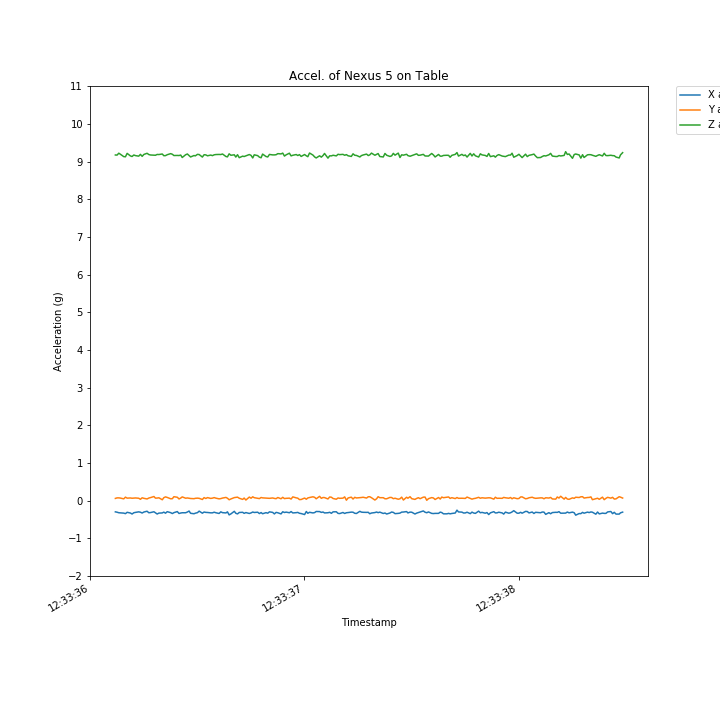
\includegraphics[scale=0.25]{won_table}
%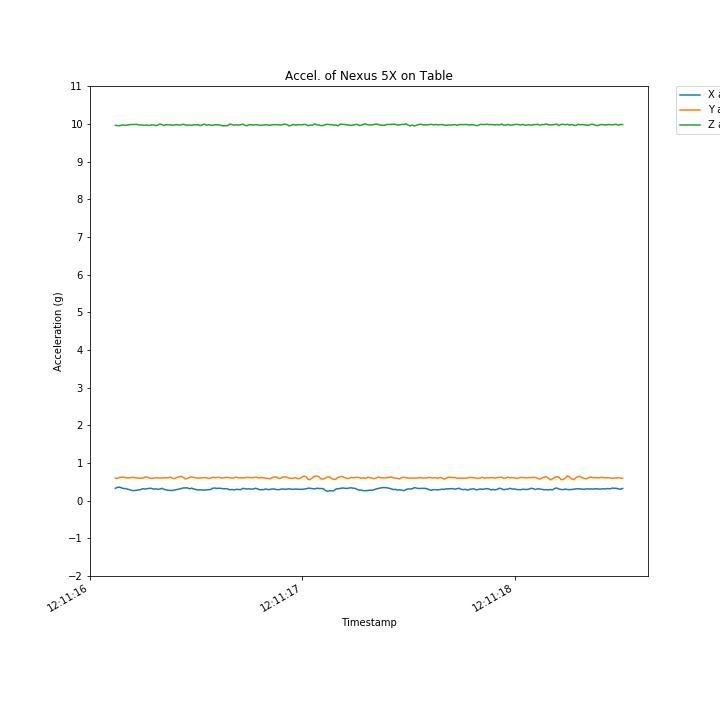
\includegraphics[scale=0.25]{joanna_table}
%\caption{Graphs of the acceleration of the Nexus 5 and 5X while on a table (at different times).}
%\end{figure}

In order to account for the inconsistent calibrations between the accelerometers of different phone models, we
attempted to recalibrate the accelerometer data for each phone before using it with the network. 
First, to see what type of recalibration model was necessary (e.g. $accel_{calibrated} = accel_{raw} + C$ or
$accel_{calibrated} = K(accel_{raw}) + C$), we taped the Nexus 5 and Nexus 5X together, and then recorded
the phones' accelerations in the four states. Plots of the two phones' accelerations against each other over the same time period
then suggested a linear relationship of the form $accel_{calibrated} = accel_{raw} + C$. 

\begin{figure*}[!h]
\center
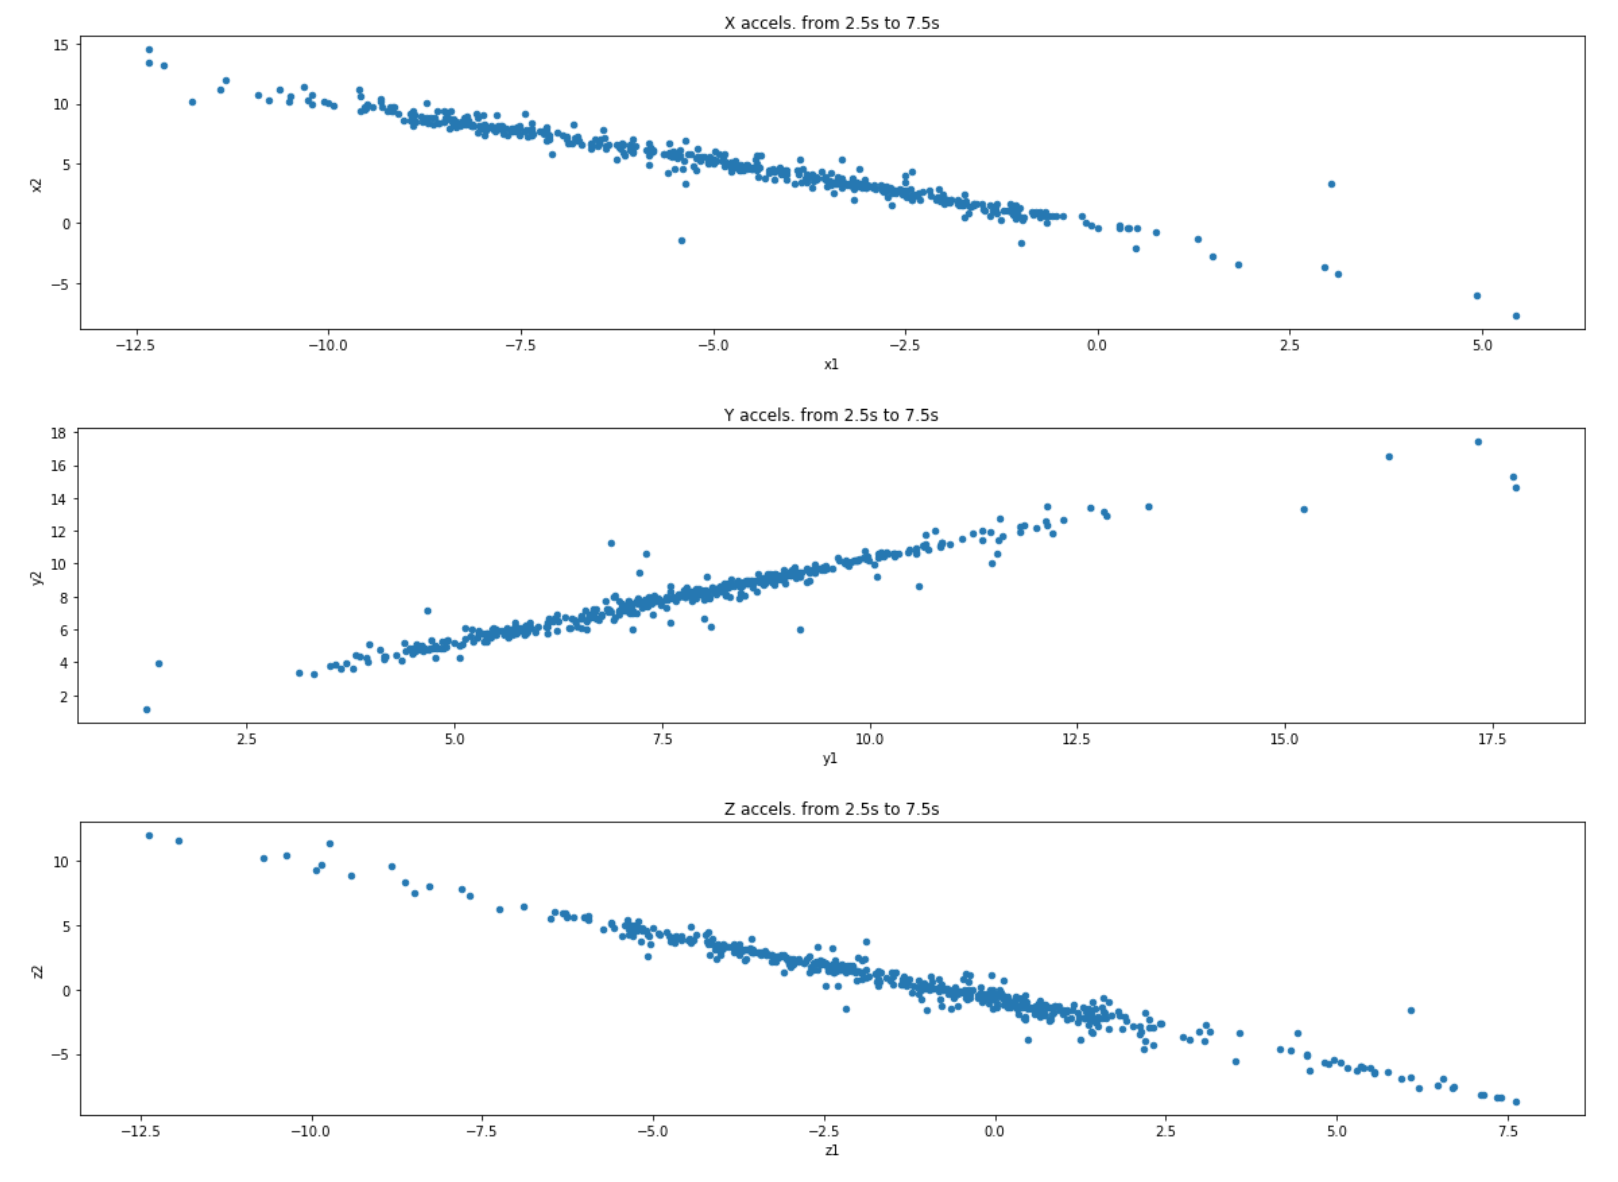
\includegraphics[scale=0.5]{two_phones}
\caption{Graphs of the acceleration of the Nexus 5X (x1/y1/z1) against the Nexus 5 (x2/y2/z2) while taped together over the same period of time.}
\end{figure*}

To find the calibration constants for each phone model, we collected accelerometer
data from when the phone was flat on a table, measured the acceleration in the
$X$, $Y$, and $Z$ directions and then computed the offsets from the expected values of
$0g$, $0g$, and $9.8g$. These offsets were then added to all of the accelerometer data for that phone model.
For practical applications of our phone state classifier, we believe that this calibration process
could then be reasonably achieved by asking phone users to place their phones flat on a table for a short period of time (e.g. a minute)
to allow the above calibration constants to be calculated.


